
\subsection{驱动因素分析}
根据气候湿润与人类活动两类驱动因素的组合,本章研究将黄河在历史时期的驱动因素变化过程分为七个时期(表\ref{tab:ch3:periods_division}),其中在公元400年之前,所有原始数据的可信度均较低,本章研究不再后续的分析中讨论(图\ref{fig:ch3:drivers}~A)。
在过去的2000年间,研究区的大多数时期均偏干燥,包括了223次极旱年和182个洪泛年的记录,因此强烈湿润的气候驱动时段并不多。
结合湿润指数,本章研究为黄河流域在过去两千年中识别了三个潜在的气候驱动期(CDPs),其中有两个在数据可靠的时期,分别开始于公元后900年与公元后1700年(图\ref{fig:ch3:drivers}~B)。
另一方面,在公元900年之前几乎没有人类活动驱动的迹象(图\ref{fig:ch3:drivers}~C)。
$900\sim1000$年间农业区域向北扩大可能指示着人类活动的增强,但因缺乏可靠的人口增长证据,且气候暖湿化也会引起农区扩张,所以此时段在本研究中不被认为是一个确定的人类活动驱动时段(HDP)。
而在这之后的1450年至1650年,以及1900年后,随着人口的显著增加和农牧交错带北移,本研究将这两个时段认为是需要分析的人类活动驱动时期(HDPs)。

% Table generated by Excel2LaTeX from sheet '历史时期特征划分'
\begin{table}[htbp]
    \centering
    \caption{基于驱动因素的历史时段划分及其特点}
      \begin{tabularx}{\textwidth}{LLL}
      \toprule
      时间跨度  & 时段划分  & 主要特征 \\
      \midrule
      200BC-400AD & 数据不可信时段 & 各数据集在此时期的可信度均偏低 \\
      400-900AD & CDP1前期 & 没有明显的驱动因素 \\
      900-1100AD & CDP1时期 & 气候驱动与低水平的人类活动驱动时期 \\
      1100-1350AD & CDP1后期 & 没有明显的驱动因素 \\
      1350-1700AD & CDP2前期 & 人类活动驱动时期 \\
      1700-1900AD & CDP2时期 & 气候驱动与人类活动共同驱动时期 \\
      1900-2000AD & HDP2时期 & 人口迅速增长的人类活动强烈驱动期 \\
      \bottomrule
      \end{tabularx}%
    \label{tab:ch3:periods_division}%
\end{table}%
  

% \begin{rotate
\begin{figure}[htb]
    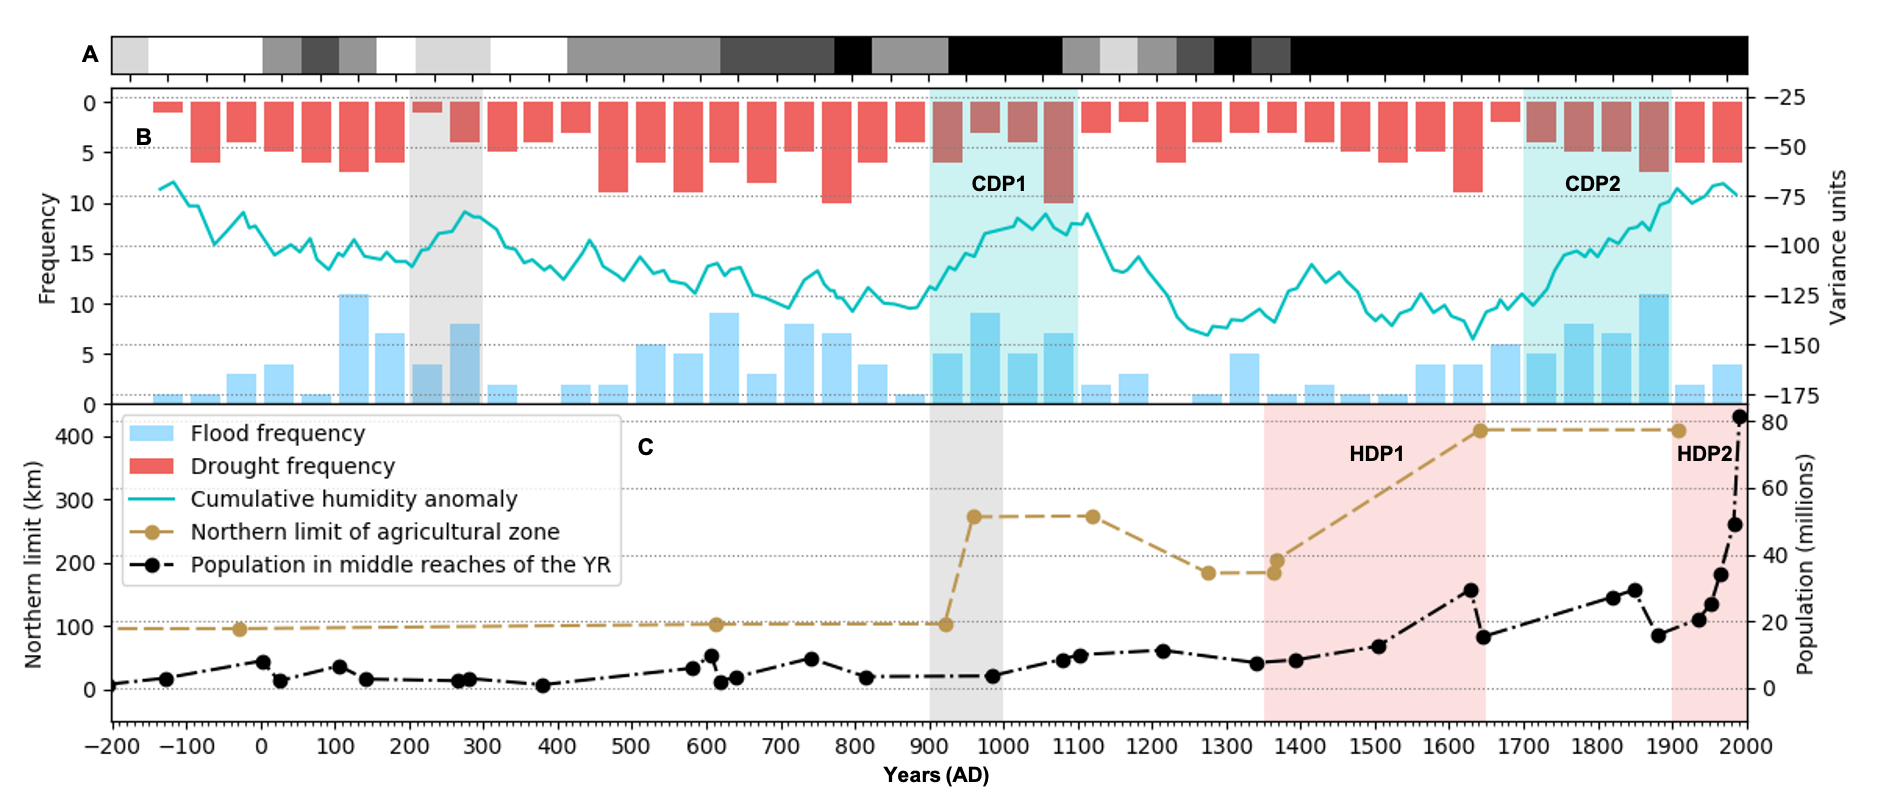
\includegraphics[width=\textwidth]{img/ch3/ch3_drivers.png}
    \caption[黄河流域历史时期稳态转换的驱动力变化]{黄河流域历史时期稳态转换的驱动力变化。
    (A) 原始数据有五级综合置信度,分别从极低置信度(白色)到极高置信度(黑色);
    (B) 气候驱动时期:用极端气候频率(干旱或洪水)以及累积湿润度距平共同确定的两个明显的气候驱动时段(CDPs),由蓝色阴影表示;
    (C) 人类活动驱动时期:根据黄河中游人口增长和农牧交错带北界的移动情况确定的人类活动驱动时段(HDPs),由红色阴影表示$^*$。}
    \footnotesize
    * 灰色阴影的部分表示农牧交错带北极界移动,但因缺乏可靠的人口增长证据且气候湿润也会引起农区扩张,所以不认为是一个人类活动驱动时段(HDP)。
    \label{fig:ch3:drivers}
\end{figure}

\subsection{影响因素分析}

根据上述时段划分,自CDP1开始(图\ref{fig:ch3:impacts}~CDP1),决溢更频繁地发生,在三门峡通航也变得更容易,同时下游两个样品的沉积速率也超过了$4cm/yr$,湿润气候驱动力带来的影响昭然若揭。
然而在CDP1之后,尽管没有沉积样品评估泥沙量,但洪泛频率的降低与重新变糟的航运情况表明,黄河的情况重新回到接近CDP1之前的时期。
最后,在时期进入第一个明显人类驱动时期(HDP1)时,更多的沉积样品表现出明显的下游泥沙沉积速率上升趋势(图\ref{fig:ch3:impacts}~HDP1$\sim$HDP2),且伴随着更频繁的洪泛与持续糟糕的航运水平。


通过结合数据置信程度,图\ref{fig:ch3:impacts}对两次气候驱动期(CDP)前、中、后期的情况提供了进一步对照。
首先,最简单直接的输沙量指标——沉积率的可信度从 HDP1 以来持续较低,在第二个人类驱动期(HDP2)结束后才有较为可靠的增加证据(图\ref{fig:ch3:impacts}~E和F)。
其次,尽管这两个潮湿的气候驱动时期均让洪泛频率明显增加(图\ref{fig:ch3:impacts}~D和E),但仅在第一个气候驱动期(CDP1)让航运更加便利,而在第二个气候驱动期结束后(CDP2,恰好也是人类活动强烈驱动期 HDP2)反而航运更加困难了。
上述对比表明,尽管气候存在周期性,但第一个强烈气候驱动期(CDP1, $900AD\sim1100AD$)与第二个气候期(CDP2, $1700AD\sim1900AD$)已呈现出不同的流域系统过程。

\begin{figure}[htb] % use float package if you want it here
    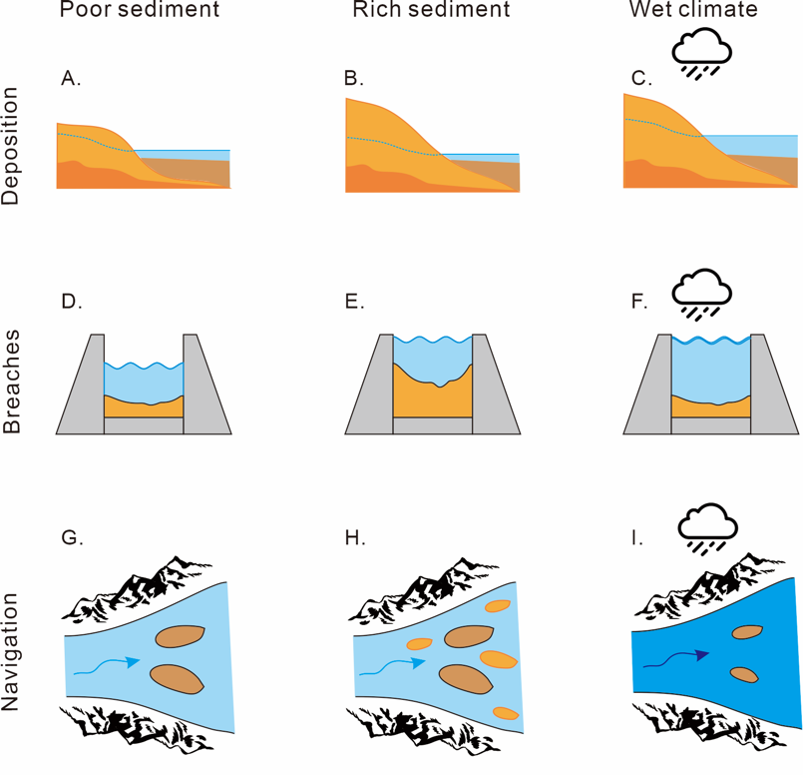
\includegraphics[width=\textwidth]{img/ch3/ch3_impacts.png}
    \caption[各时段的影响因素及其可信度的整合分析。]{各时段的影响因素及其可信度的整合分析。每个时段内(气候驱动时段CDP,或人类活动驱动时段HDP),沉积(黄色)、洪泛(蓝色)、航运(红色)三个典型受影响因素的特征等级与可信度等级(见\ref{sec:ch3:approach}\nameref{sec:ch3:approach})。在每个半圆内,扇形的半径表明影响因素的强度等级,弧长表示其数据可信度。由于航运和洪泛滥同水量变化是相反的,本章研究将它们放在扇形的不同象限,从而使扇形左右两个方向分别代表更少的水量与更多的水量。简而言之,某个颜色的扇形面积更大,就有越大的把握说明该时段内的此影响因素强度。$A \sim F$分别代表被两次气候驱动期CDP所分割的不同时段:(A.) 400AD-900AD; (B.) 900AD-1100AD; (C.) 1100AD-1350AD; (D.) 1350AD-1700AD; (E.) 1700AD-1900AD; 和(F.)1900AD-2000AD。}\label{fig:ch3:impacts}
\end{figure}

\subsection{发生过程总结}
首先,本章研究检测到的驱动力时段(两个气候驱动和两个人类活动驱动)均能够在既有研究中得到印证。
(1)从900年到公元1100年的CDP1是一个典型的潮湿时期,通常被称为“中世纪暖期” \cite{zhang1993, zhang1994, man2014},此时期温暖而潮湿的气候让通常会引发农业范围的北扩\cite{TanQiXiang1996,GeQuanSheng2011}。
(2)第二个气候驱动期(公元1700年到1900年,CDP2)几乎覆盖了整个中国古代清朝,包括此时开始的我国最早的系统性气象观测资料——“雨雪分寸”在内的各种数据反演结果都能表明,这是一个典型的湿期\cite{hao2021, ge2008}。
(3)本章研究识别的第一个人类活动驱动时期持续时间较长(公元1350年至公元1650年,HDP1),而根据 Wang 等人的考证,这段时间靠中间的公元1491年,黄土高原人口迅速增加到1150万,且有着土地复垦加速的可信记录\cite{wang2006b}。
(4)第二个人类活动驱动时期(1900以后,HDP2)已是近代,史料较为丰富切翔实可靠,期间除了快速增长的人口也记录了频繁的土地纠纷,以及黄河中游强烈的开垦和农业土地利用\cite{GeJianXiong2005}。
其次,影响因素的组合作为识别稳态转换过程的潜在参考,能展示更多关于变化时期的信息,同样也得到了前人研究的佐证。
在潮湿的气候驱动期,增加的降水同时提升了洪泛频次、土壤侵蚀、与泥沙沉积\cite{chen2012}。
此外,此时期的湿润气候也有利于三门峡谷通行,而这正是北宋政府沿着黄河水路运输的粮食的关键\cite{WangShouChun1993}。

通过结合上述驱动力和影响,本章研究可以在千年尺度上对黄河如何进入受人类活动主导的稳态做如下解释。
首先,在潮湿的第一个气候驱动时期中发生的变化(即沉积速率增加,更频繁的洪泛,以及航运得到改善)在此时期后,仅沉积速率保持相对不变(可能源于由于有限的农业扩张,但数据可信度较弱),而航运情况与洪泛情况都重新回到此时期前的水平。
因此,尽管潮湿的气候与人类活动都有所体现,但此时期仍然是气候变化为主要驱动力,且稳态转换的临界点没有达到(图\ref{fig:ch3:regime_shift}~A)。
接下来开始的人类活动驱动时期(HDP)期间,持续增强的开垦压力导致影响因素的组合产生了一些差异(见图\ref{fig:ch3:impacts}~从C到D),因此在CDP2期间,潮湿的气候仅影响洪水的频率而已无法缓解困难的三门峡通航情况。
最后,在第二个气候驱动期(CDP2)也结束之后也迎来了新的人类活动驱动期(HDP2),仅有洪泛频率退回到潮湿期之前的水平,泥沙沉积速率仍在增加,通航状况也到了历史最糟糕的时期,所有这些迹象表明稳态转换已经发生,人类活动已经主导了黄河流域,源自1350年以来不断增加的人为压力将稳态推出了气候周期规律(图\ref{fig:ch3:regime_shift}~B)。

\begin{figure}[htb] % use float package if you want it here
    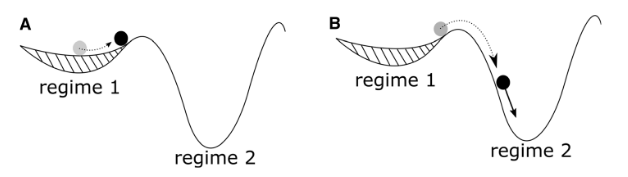
\includegraphics[width=\textwidth]{img/ch3/ch3_regime_shift.png}
    \caption[黄河流域转向人类活动主导的稳态转换过程解释图]{黄河流域转向人类活动主导的稳态转换过程解释图。Regime1 和 Regime2 分别表示原始状态下自然驱动力主导的黄河与人类活动主导的黄河。灰色的圆圈用虚线箭头表示流域系统在气候驱动力下的状态。黑色圆实心箭头表示不断增强的人为压力。A图所示的变化反映了从400年到1350年的过程(对应于图\ref{fig:ch3:impacts}的从A到C)。B图所示的变化为从1350年到公元2000年(对应于图\ref{fig:ch3:impacts}的从D到F)。}
    \label{fig:ch3:regime_shift}
\end{figure}
